\chapter{ทบทวนความรู้พื้นฐานทางเรขาคณิต}

\begin{agreementbox}
สัญลักษณ์ต่าง ๆ ตลอดเนื้อหาของเอกสารฉบับนี้ มีความหมายดังนี้
\begin{enumerate}
\item สัญลักษณ์ $\times$ และ $\cdot$ หมายถึง เครื่องหมายคูณ
    \item สัญลักษณ์ $\angle A$ หรือ $\hat{A}$ หมายถึง ขนาดของมุม $A$
    \item สัญลักษณ์ $\triangle ABC$ หมายถึง สามเหลี่ยม $ABC$ และ $[\triangle ABC]$ หมายถึง พื้นที่ของ $\triangle ABC$
    \item สัญลักษณ์ $\square ABCD$ หมายถึง สี่เหลี่ยม $ABCD$ และ $[\square ABCD]$ หมายถึง พื้นที่ของ $\square ABCD$
    \item ให้ $\ell_1$ และ $\ell_2$ แทนเส้นตรงสองเส้น สัญลักษณ์ $\ell_1 // \ell_2$ หมายถึง เส้นตรง $\ell_1$ และ $\ell_2$ ขนานกัน
\end{enumerate} 
\end{agreementbox}

\begin{theorembox}
กำหนดให้ $\triangle ABC$ เป็นสามเหลี่ยมมุมฉาก โดยมีความยาวด้านต่าง ๆ แสดงดังรูปที่~\ref{Figure12}\\
เราได้ว่า
\[a^2+b^2=c^2\]
\end{theorembox}
 \begin{figure}[H]	
	\centering
	\includegraphics[scale=0.5]{12}
    	\caption{}
       \label{Figure12}
\end{figure} 


\section{จุด เส้นตรงและมุม}
\begin{remarkbox}
จากจุดจุดหนึ่งภายนอกเส้นตรง สามารถลากเส้นตั้งฉากกับเส้นตรงที่กำหนดให้\\
จากรูปที่~\ref{Figure61} เราสามารถลากเส้นจากจุด $X$ มาตั้งฉากกับเส้นตรง $\ell$ ได้
\end{remarkbox}
 \begin{figure}[H]	 
	\centering
	\includegraphics[scale=0.65]{61}
    	\caption{}
       \label{Figure61}
\end{figure} 

\begin{remarkbox}
ถ้ามุมสองมุมอยู่ในแนวเส้นตรงเดียวกัน แล้วมุมทั้งสองนั้นจะเป็นมุมประกอบสองมุมฉาก\\
จากรูปที่~\ref{Figure41} สามารถสรุปได้ว่า
\[\alpha+\beta=180^{\circ}\]
\end{remarkbox}
 \begin{figure}[H]	 
	\centering
	\includegraphics[scale=0.65]{41}
    	\caption{}
       \label{Figure41}
\end{figure} 

\newpage
\begin{definitionbox}
เส้นตรงสองเส้น \textbf{ขนานกัน} ก็ต่อเมื่อ เส้นตรงสองเส้นนั้นอยู่บนระนาบเดียวกันและไม่ตัดกัน \\
จากรูปที่~\ref{Figure59} แสดงเส้นตรง $\ell_1 // \ell_2$
\end{definitionbox}

 \begin{figure}[H]	 
	\centering
	\includegraphics[scale=0.65]{59}
    	\caption{}
       \label{Figure59}
\end{figure} 

\begin{remarkbox}
เส้นตรงสองเส้นตัดมุมตรงข้ามย่อมเท่ากัน\\
จากรูปที่~\ref{Figure60} แสดงเส้นตรง $\ell_1$ และ $\ell_2$ ตัดกัน สามารถสรุปได้ว่า
\[\alpha=\beta\]
\end{remarkbox}
 \begin{figure}[H]	 
	\centering
	\includegraphics[scale=0.65]{60}
    	\caption{}
       \label{Figure60}
\end{figure} 

\newpage
\begin{remarkbox}
ถ้าเส้นตรงสองเส้นถูกตัดด้วยเส้นตรงเส้นหนึ่งที่ทำให้มุมแย้งเท่ากัน แล้วเส้นตรงคู่นั้นจะขนานกัน\\
จากรูปที่~\ref{Figure49} เส้นตรง $\ell_1$ และ $\ell_2$ ถูกตัดด้วยเส้นตรง $\ell$ ที่ทำให้ $\alpha=\beta$ สามารถสรุปได้ว่า
\[\ell_1 // \ell_2\]
\end{remarkbox}
 \begin{figure}[H]	 
	\centering
	\includegraphics[scale=0.6]{49}
    	\caption{}
       \label{Figure49}
\end{figure} 
\newpage
\begin{theorembox}
เมื่อเส้นตรงเส้นหนึ่งตัดเส้นตรงคู่หนึ่ง ถ้าเส้นตรงคู่นี้ \textbf{ขนานกัน} แล้ว
\begin{enumerate}
\item มุมแย้งเท่ากัน
\item มุมภายนอกและมุมภายในที่อยู่ตรงข้ามบนข้างเดียวกันของเส้นตัดมีขนาดเท่ากัน
\item มุมภายในที่อยู่ข้างเดียวกันของเส้นตัดรวมกันเท่ากับสองมุมฉาก
\end{enumerate}
จากรูปที่~\ref{Figure40} กำหนดให้เส้นตรง $\ell$ ตัดกับเส้นตรง $\ell_1$ และ $\ell_2$ ที่ขนานกัน สามารถสรุปได้ว่า
\begin{enumerate}
\item $\hat{4}=\hat{5}$ และ $\hat{2}=\hat{6}$
\item $\hat{1}=\hat{2},\quad \hat{3}=\hat{4},\quad \hat{5}=\hat{8}$ และ $\hat{6}=\hat{7}$
\item $\hat{2}+\hat{5}=180^{\circ}$ และ $\hat{4}+\hat{6}=180^{\circ}$
\end{enumerate}
\end{theorembox}
 \begin{figure}[H]	 
	\centering
	\includegraphics[scale=0.55]{40}
    	\caption{}
       \label{Figure40}
\end{figure} 
\newpage


\begin{figure}[H]	 
	\centering
	\includegraphics[scale=0.5]{39}
    	\caption{}
       \label{Figure39}
\end{figure} 

\newpage
\section{วงกลม}
\begin{theorembox}
มุมในครึ่งวงกลมเป็นมุมฉาก\\
จากรูปที่~\ref{Figure1} เราได้ว่า $\angle ABC=90^{\circ}$
\end{theorembox}
 \begin{figure}[H]	
	\centering
	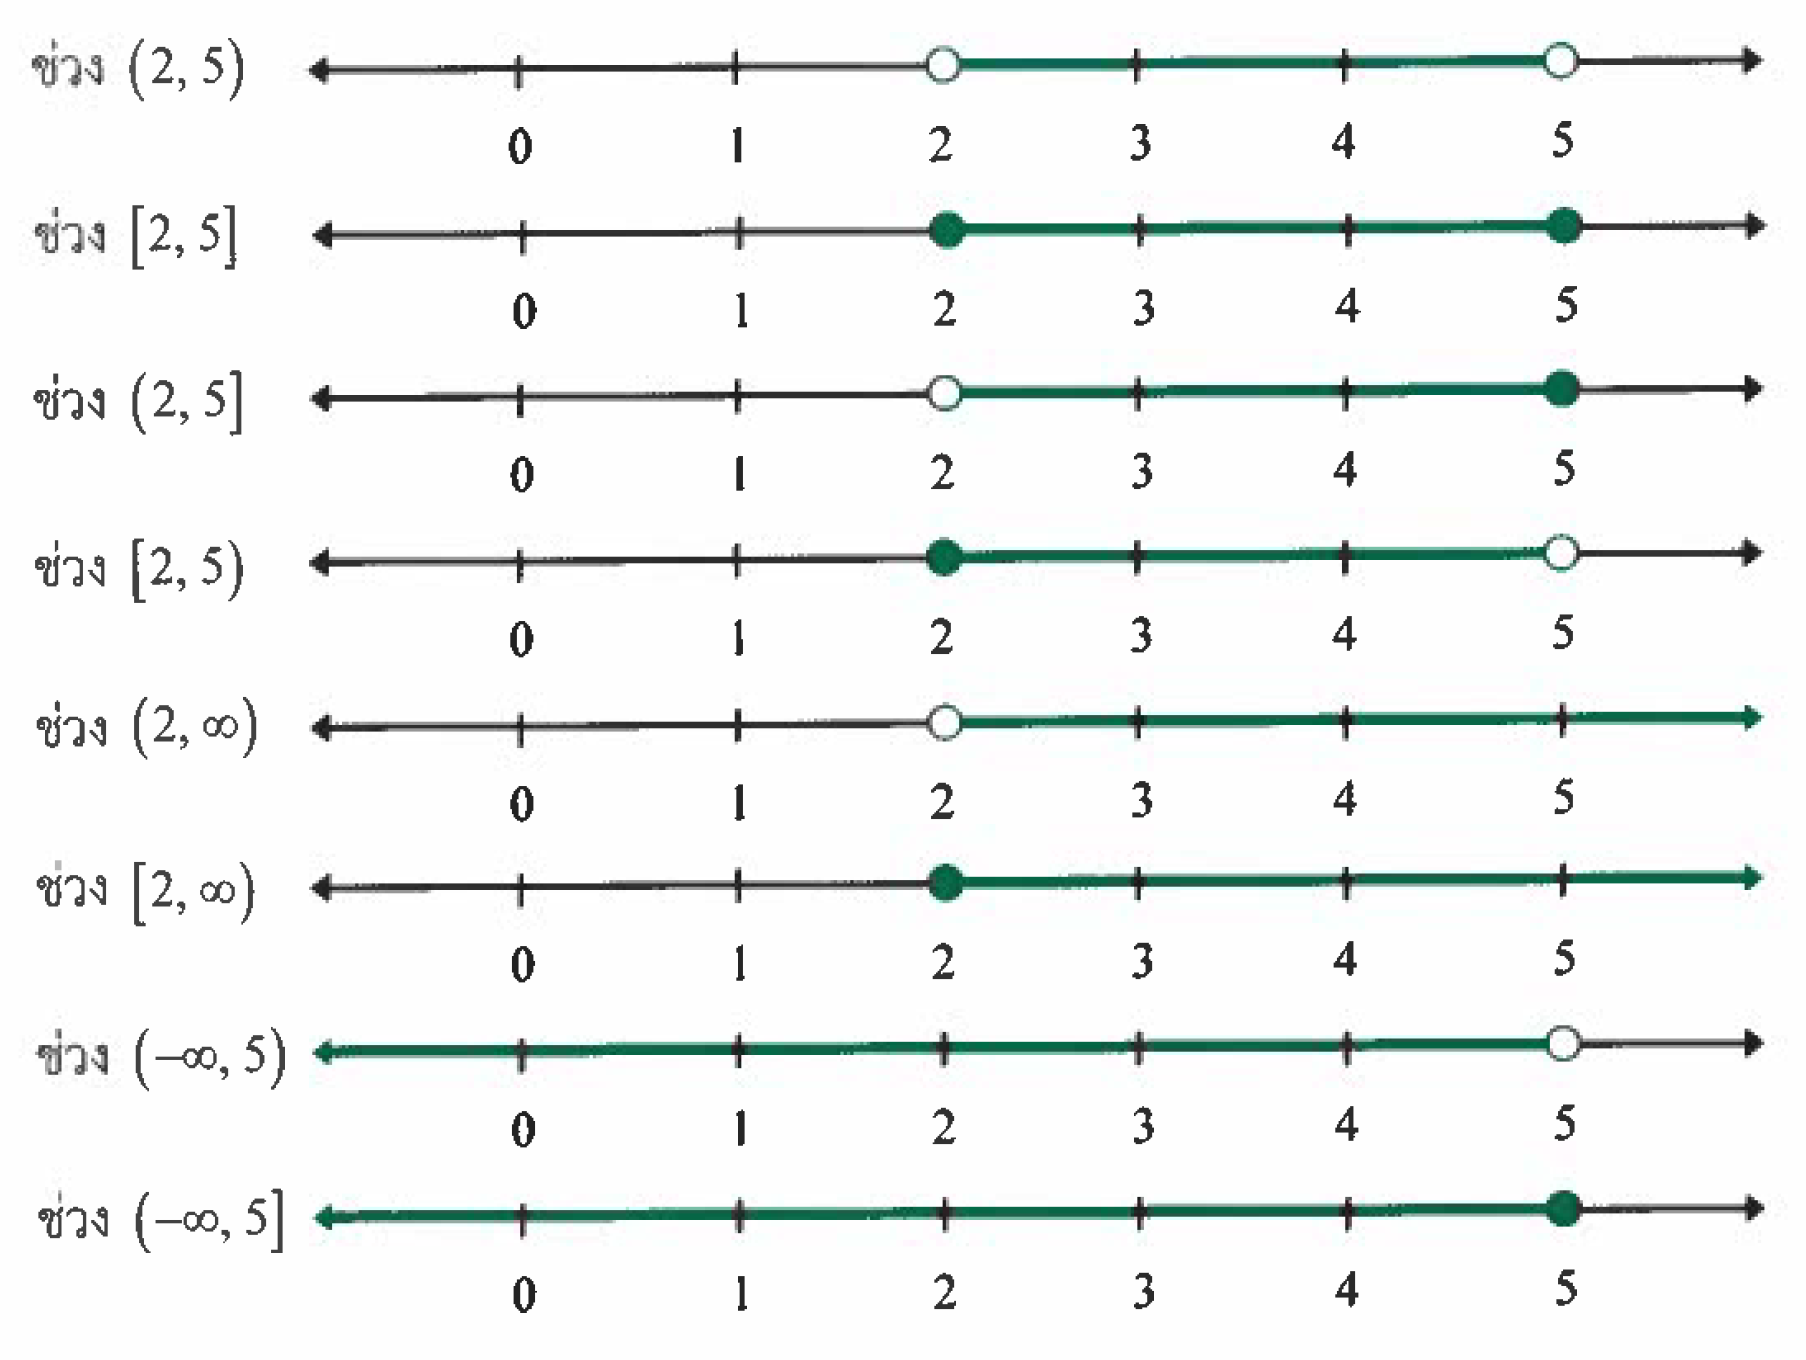
\includegraphics[scale=0.5]{1}
    	\caption{}
       \label{Figure1}
\end{figure} 

\begin{theorembox}
ถ้ามุมที่จุดศูนย์กลางของวงกลมและมุมในส่วนโค้งของวงกลมรองรับด้วยส่วนโค้งเดียวกันแล้ว มุมที่จุดศูนย์กลางของวงกลมมีขนาดเป็นสองเท่าของมุมในส่วนโค้งของวงกลม\\
จากรูปที่~\ref{Figure2} เราได้ว่า $\angle AOB=2\angle ACB$
\end{theorembox}
 \begin{figure}[H]	
	\centering
	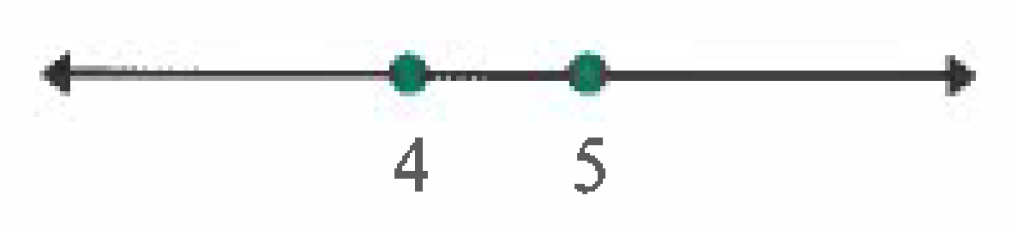
\includegraphics[scale=0.5]{2}
    	\caption{}
       \label{Figure2}
\end{figure} 

\begin{theorembox}
มุมในส่วนของวงกลมเดียวกันย่อมเท่ากัน\\
จากรูปที่~\ref{Figure3} เราได้ว่า $B\hat{A}C=B\hat{D}C$
\end{theorembox}
 \begin{figure}[H]	
	\centering
	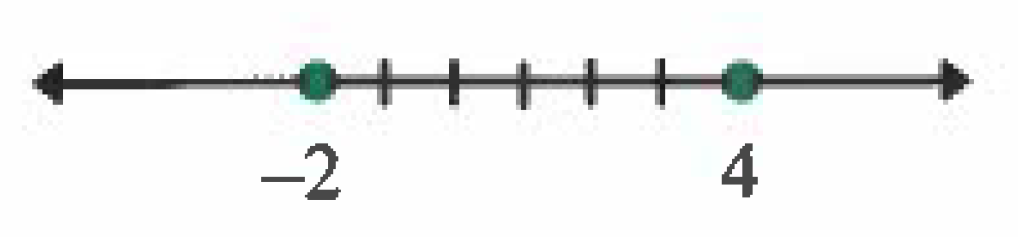
\includegraphics[scale=0.5]{3}
    	\caption{}
       \label{Figure3}
\end{figure} 

\begin{examplebox}[NETSAT คณิตศาสตร์ สิงหาคม 2568]
จากรูปที่~\ref{Figure4} กำหนดให้ $A,B$ และ $C$ อยู่บนเส้นรอบวงของวงกลม และ $\angle  OBC=39^{\circ}$ แล้วมุม $x$ มีขนาดเท่าใด
\begin{multicols}{2} \begin{enumerate}
\item $39^{\circ}$
\item $51^{\circ}$
\item $78^{\circ}$
\item $102^{\circ}$
\end{enumerate} \end{multicols}
\end{examplebox}
 \begin{figure}[H]	 
	\centering
	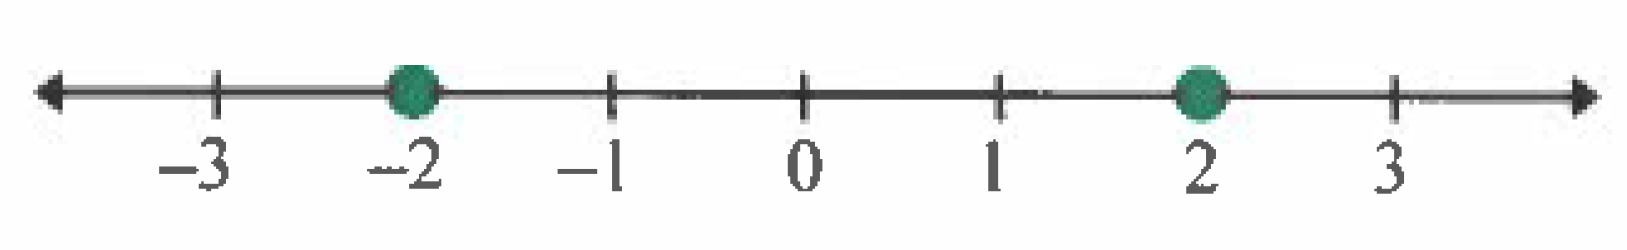
\includegraphics[scale=0.6]{4}
    	\caption{}
       \label{Figure4}
\end{figure} 

\newpage
\begin{examplebox}[NETSAT คณิตศาสตร์ สิงหาคม 2565]
จากรูปที่~\ref{Figure5} กำหนดให้จุด $A, B, C$ และ $D$ อยู่บนเส้นรอบวงของวงกลม ให้ $E$ เป็นจุดตัดของ $A C$ และ $B D$ เมื่อ $\angle A E D=112^{\circ}$ และ $\angle E D C=31^{\circ}$ แล้ว $\angle A B E$ เท่ากับข้อใด
\begin{multicols}{2} \begin{enumerate}
\item $37^{\circ}$
\item $68^{\circ}$
\item $81^{\circ}$
\item $ 99^{\circ}$
\end{enumerate} \end{multicols}
\end{examplebox}
 \begin{figure}[H]	 
	\centering
	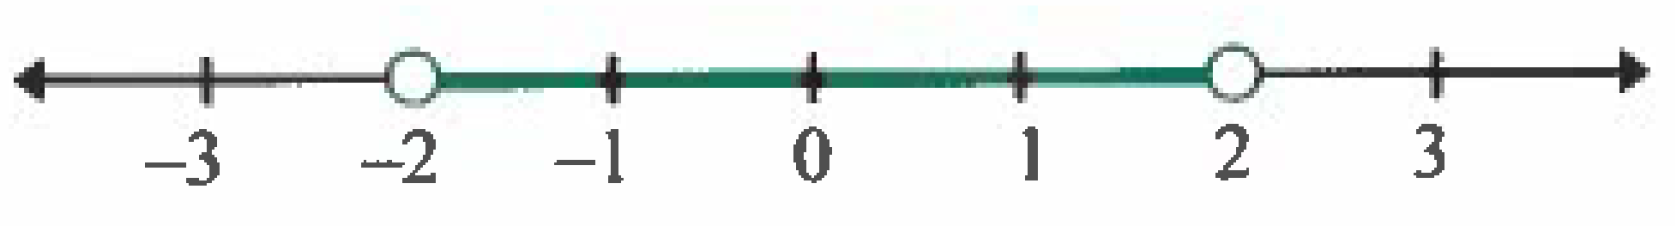
\includegraphics[scale=0.8]{5}
    	\caption{}
       \label{Figure5}
\end{figure} 
\newpage
\begin{examplebox}[NETSAT คณิตศาสตร์ กุมภาพันธ์ 2565]
หน้าปัดนาพิกาถูกแบ่งเป็น $60$ ส่วนเท่า ๆ กัน (ดังแสดงในรูปที่~\ref{Figure55}) ให้ $A, B$ และ $C$ เป็นจุดอยู่ ที่ $9,6$ และ $5$ นาพิกา ตามลำดับ (ดังแสดงในรูปที่~\ref{Figure56}) สมมติว่าจุดทั้งสามจุดนี้อยู่บนเส้นรอบวงของวงกลม $O$ แล้ว $\angle BAC$ มีค่าเท่าใด
\begin{multicols}{2} \begin{enumerate}
\item $10^{\circ}$
\item $15^{\circ}$
\item $20^{\circ}$
\item $30^{\circ}$
\end{enumerate} \end{multicols}
\end{examplebox}
 \begin{figure}[H]	 
\centering
	\includegraphics[scale=0.5]{55}
    	\caption{}
       \label{Figure55}
\end{figure} 
 \begin{figure}[H]	 
	\centering
	\includegraphics[scale=0.5]{56}
    	\caption{}
       \label{Figure56}
\end{figure} 
\newpage


\begin{theorembox}
จากรูปที่~\ref{Figure7} คอร์ด $AB$ และคอร์ด $CD$ ตัดกันที่จุด $X$ เราได้ว่า
\[XA\cdot XB = XC\cdot XD\]
\end{theorembox}
 \begin{figure}[H]	
	\centering
	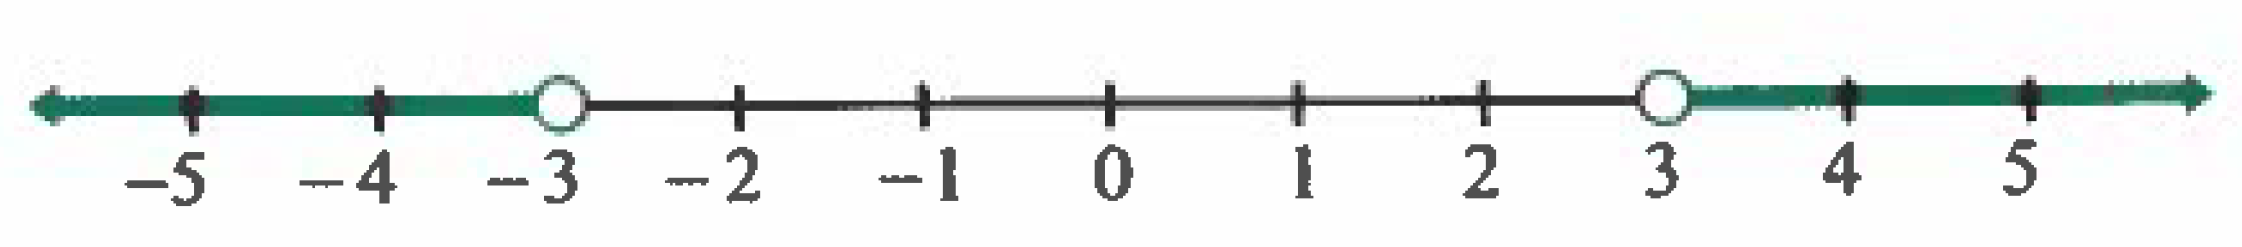
\includegraphics[scale=0.5]{7}
    	\caption{}
       \label{Figure7}
\end{figure} 

\begin{examplebox}[NETSAT คณิตศาสตร์ 2566]
กำหนดให้ คอร์ด $AB$ และคอร์ด $CD$ ตัดกันดังรูปที่~\ref{Figure8} จงหาว่า $x$ มีค่าเท่าใด
\begin{multicols}{2} \begin{enumerate}
\item $2$
\item $2.5$
\item $3.6$
\item $4$
\end{enumerate} \end{multicols}
\end{examplebox}
 \begin{figure}[H]	 
	\centering
	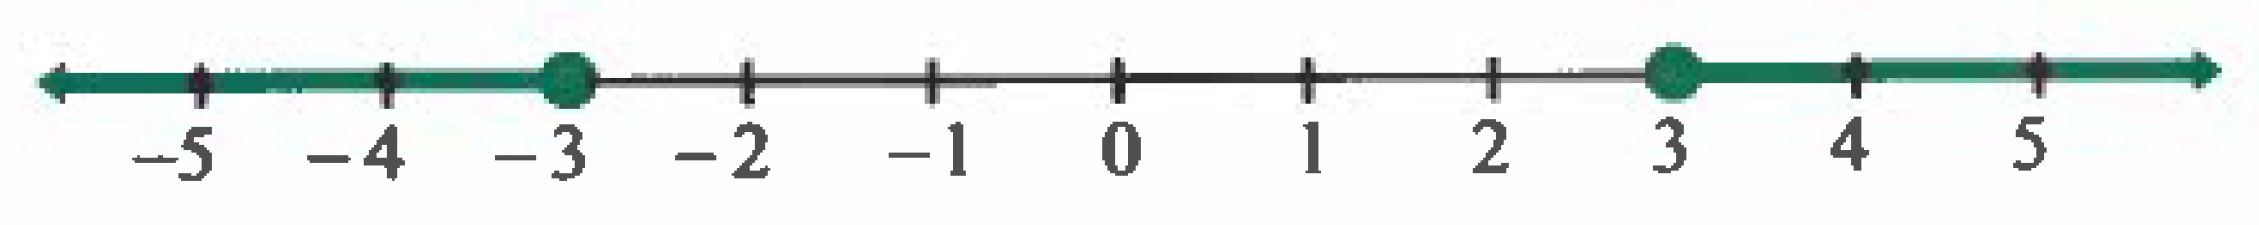
\includegraphics[scale=0.55]{8}
    	\caption{}
       \label{Figure8}
\end{figure} 

\newpage

\begin{examplebox}[NETSAT คณิตศาสตร์ กุมภาพันธ์ 2565]
กำหนดให้ คอร์ด $AB$ และคอร์ด $CD$ ตัดกันดังรูปที่~\ref{Figure9} จงหาว่า $x$ มีค่าเท่าใด
\begin{multicols}{2} \begin{enumerate}
\item $9$
\item $12$
\item $\dfrac{16}{3}$
\item $\dfrac{3}{4}$
\end{enumerate} \end{multicols}
\end{examplebox}
 \begin{figure}[H]	 
	\centering
	\includegraphics[scale=0.9]{9}
    	\caption{}
       \label{Figure9}
\end{figure} 

\newpage

\begin{theorembox}
ขนาดของมุมที่อยู่ตรงข้ามของรูปสี่ด้านที่แนบในวงกลมรวมกันแล้วเท่ากับสองเท่าของมุมฉาก\\
จากรูปที่~\ref{Figure10} กำหนดให้ $\square ABCD$ แนบในวงกลม เราได้ว่า $\alpha_1+\beta_1=180^{\circ}$ และ $\alpha_2+\beta_2=180^{\circ}$
\end{theorembox}
 \begin{figure}[H]	
	\centering
	\includegraphics[scale=0.55]{10}
    	\caption{}
       \label{Figure10}
\end{figure} 

\begin{examplebox}[NETSAT คณิตศาสตร์ สิงหาคม 2565]
 $\square A B C D$ บรรจุในวงกลม โดยที่ $\angle A E D=75^{\circ}$ และ $\angle B C D=130^{\circ}$ ซึ่งแสดงดังรูปที่~\ref{Figure11} แล้วมุม $x$ มีค่าเท่าใด
\begin{multicols}{2} \begin{enumerate}
\item $80^{\circ}$
\item $100^{\circ}$
\item $105^{\circ}$
\item $110^{\circ}$
\end{enumerate} \end{multicols}
\end{examplebox}
 \begin{figure}[H]	 
	\centering
	\includegraphics[scale=0.55]{11}
    	\caption{}
       \label{Figure11}
\end{figure} 


\begin{theorembox}\label{theorem1.7}
ถ้าลากส่วนของเส้นตรงจากจุดศูนย์กลางของวงกลมไป \textbf{แบ่งครึ่ง} คอร์ดซึ่งไม่ผ่านจุดศูนย์กลาง ส่วนของเส้นตรงนั้นจะตั้งฉากกับคอร์ด\\
จากรูปที่~\ref{Figure57} เราได้ว่า $OC$ ตั้งฉากกับ 
\end{theorembox}
 \begin{figure}[H]	 
	\centering
	\includegraphics[scale=0.55]{57}
    	\caption{}
       \label{Figure57}
\end{figure} 
\begin{theorembox}[บทกลับของทฤษฎี~\ref{theorem1.7}]
ถ้าลากส่วนของเส้นตรงจากจุดศูนย์กลางของวงกลมไป \textbf{ตั้งฉาก} กับคอร์ดซึ่งไม่ผ่านจุดศูนย์กลาง ส่วนของเส้นตรงนั้นจะแบ่งครึ่งคอร์ด\\
จากรูปที่~\ref{Figure24} เราได้ว่า $AC=CB$
\end{theorembox}
 \begin{figure}[H]	 
	\centering
	\includegraphics[scale=0.55]{24}
    	\caption{}
       \label{Figure24}
\end{figure} 
\newpage

\begin{examplebox}[NETSAT คณิตศาสตร์ สิงหาคม 2565]
จากรูปที่~\ref{Figure18} กำหนดให้วงกลมมีจุดศูนย์กลางที่จุด $O$ และมีความยาวคอร์ด $AB$ เท่ากับ $6$ เซนติเมตร และระยะจากจุด $O$ ถึงคอร์ด $AB$ เท่ากับ $2$ เซนติเมตร จงหาความยาวรัศมีวงกลม
\begin{multicols}{2} \begin{enumerate}
\item $\sqrt{11}$
\item $\sqrt{13}$
\item $4$
\item $5$
\end{enumerate} \end{multicols}
\end{examplebox}
 \begin{figure}[H]	 
	\centering
	\includegraphics[scale=0.8]{18}
    	\caption{}
       \label{Figure18}
\end{figure} 
\newpage

\subsection{เส้นสัมผัสวงกลม}
\begin{remarkbox}
\begin{enumerate}
\item \textbf{เส้นสัมผัสวงกลม} คือ เส้นตรงซึ่งตัดวงกลมเพียงจุดเดียวเท่านั้น
\item จากจุดจุดหนึ่งภายนอกวงกลม ลากเส้นสัมผัสมายังวงกลมได้เพียงสองเส้นเท่านั้น และ \textbf{เส้นสัมผัสนั้นยาวเท่ากัน}
\item เส้นสัมผัส \textbf{ตั้งฉาก} กับเส้นรัศมีซึ่งลากมาที่จุดสัมผัส
\end{enumerate}
จากรูปที่~\ref{Figure32} เราได้ว่า $\angle OCB= \angle OAB = 90^{\circ}$ และ $AB=CB$ 
\end{remarkbox}
 \begin{figure}[H]	 
	\centering
	\includegraphics[scale=0.65]{32}
    \caption{}
    \label{Figure32}
\end{figure} 

\newpage
\begin{remarkbox}
รูปสามเหลี่ยมที่มีด้านยาวเท่ากันสองด้านและมุมที่ฐานมีขนาดเท่ากันเรียกว่า \textbf{รูปสามเหลี่ยมหน้าจั่ว}\\
จากรูปที่~\ref{Figure34} เราได้ว่า $AB=AC$ และ $\angle ABC= \angle ACB$ 
\end{remarkbox}
 \begin{figure}[H]	 
	\centering
	\includegraphics[scale=0.45]{34}
    \caption{}
    \label{Figure34}
\end{figure} 

\begin{theorembox}
มุมที่เกิดจากเส้นสัมผัสจดกับคอร์ดย่อมเท่ากับมุมที่อยู่ในส่วนของวงกลมตรงกันข้าม\\
จากรูปที่~\ref{Figure33} เราได้ว่า 
\[\angle BAC = \angle DBC\]
\end{theorembox}
 \begin{figure}[H]	 
	\centering
	\includegraphics[scale=0.5]{33}
    \caption{}
    \label{Figure33}
\end{figure} 

\newpage
\begin{examplebox}[NETSAT คณิตศาสตร์ สิงหาคม 2568]
จากรูปที่~\ref{Figure31} จงหา $\angle BCD$
\begin{multicols}{2} \begin{enumerate}
\item $71^{\circ}$
\item $72^{\circ}$
\item $73^{\circ}$
\item $74^{\circ}$
\end{enumerate} \end{multicols}
\end{examplebox}
 \begin{figure}[H]	 
	\centering
	\includegraphics[scale=0.7]{31}
    	\caption{}
       \label{Figure31}
\end{figure} 

\newpage
\section{พื้นที่สามเหลี่ยม, สี่เหลี่ยม และวงกลม}
\subsection{พื้นที่สามเหลี่ยม}
\begin{remarkbox}
กำหนดให้ $\triangle ABC$ แสดงดังรูปที่~\ref{Figure42},~\ref{Figure43} และ~\ref{Figure44} ตามลำดับ เราจะได้ว่าพื้นที่ของ $\triangle ABC$ หาได้จาก
\[[\triangle ABC]=\frac{1}{2}\times h \times AB\]
\end{remarkbox}
 \begin{figure}[H]	
	\centering
	\includegraphics[scale=0.5]{42}
    	\caption{}
       \label{Figure42}
\end{figure} 
 \begin{figure}[H]	
	\centering
	\includegraphics[scale=0.5]{43}
    	\caption{}
       \label{Figure43}
\end{figure} 
 \begin{figure}[H]	
	\centering
	\includegraphics[scale=0.5]{44}
    	\caption{}
       \label{Figure44}
\end{figure} 

\subsection{พื้นที่วงกลม}
\begin{remarkbox}
กำหนดให้วงกลมมีจุดศูนย์กลางที่จุด $O$ และมีรัศมี $r$ หน่วย แสดงดังรูปที่~\ref{Figure45} \\
เราจะได้ว่าพื้นที่ของวงกลมหาได้จาก
\[\pi\times r^2\]
และความเส้นรอบวงกลมหาได้จาก 
\[2\times \pi\times r\]
\end{remarkbox}
 \begin{figure}[H]	
	\centering
	\includegraphics[scale=0.55]{45}
    	\caption{}
       \label{Figure45}
\end{figure} 

\newpage
\subsection{พื้นที่สี่เหลี่ยม}
\begin{remarkbox}
กำหนดให้ $\square ABCD$ เป็นรูปสี่เหลี่ยมผืนผ้า หรือ รูปสี่เหลี่ยมจัตุรัส แสดงดังรูปที่~\ref{Figure46} \\
เราจะได้ว่า
\[[\square ABCD]=xy\]
\end{remarkbox}
 \begin{figure}[H]	
	\centering
	\includegraphics[scale=0.55]{46}
    	\caption{}
       \label{Figure46}
\end{figure} 

\begin{remarkbox}
กำหนดให้ $\square ABCD$ เป็นรูปสี่เหลี่ยมคางหมู แสดงดังรูปที่~\ref{Figure47} \\
เราจะได้ว่า
\[[\square ABCD]=\frac{1}{2}\times (x+y)\times h\]
\end{remarkbox}
 \begin{figure}[H]	
	\centering
	\includegraphics[scale=0.55]{47}
    	\caption{}
       \label{Figure47}
\end{figure} 
\newpage
\noindent จากรูปที่~\ref{Figure16} วงกลม $P$ มีรัศมี $2 \sqrt{5}$ เซนติเมตร และวงกลม $Q$ มีรัศมี $\sqrt{5}$ เซนติเมตร วงกลม $P$ และ $Q$ สัมผัสกัน และวงกลมทั้งสองสัมผัสกับส่วนของเส้นตรง (ตั้งฉากซึ่งกัน และตั้งฉากกับส่วนของเส้นตรง $\ell$ กำหนดให้ $A$ และ $B$ เป็นจุดตัดของส่วนของเส้นตรง $\ell$ และเส้นตั้งฉากที่ลากจากจุดศูนย์กลางวงกลม $P$ และ $Q$ มาที่เส้นตรง $\ell$\\
จากข้อมูลดังกล่างให้ใช้ตอบคำถามตัวอย่าง~\ref{example1.10} และตัวอย่าง~\ref{example1.11}
 \begin{figure}[H]	 
	\centering
	\includegraphics[scale=0.65]{16}
    	\caption{}
       \label{Figure16}
\end{figure} 

\begin{examplebox}[NETSAT คณิตศาสตร์ 2566] \label{example1.10}
จากรูปที่~\ref{Figure16} ข้อใดคือผลรวมของพื้นที่ของวงกลม $P$ และวงกลม $Q$
\begin{multicols}{2} \begin{enumerate}
\item $15 \pi$ ลูกบาศก์เซนติเมตร
\item $25 \pi$ ลูกบาศก์เซนติเมตร
\item $35 \pi$ ลูกบาศก์เซนติเมตร
\item $45 \pi$ ลูกบาศก์เซนติเมตร
\end{enumerate} \end{multicols}
\end{examplebox}


\begin{examplebox}[NETSAT คณิตศาสตร์ 2566]\label{example1.11}
จากรูปที่~\ref{Figure16} จะหาความยาวของส่วนเส้นตรง $A B$
\begin{multicols}{2} \begin{enumerate}
\item $3 \sqrt{5}$ เซนติเมตร
\item $4 \sqrt{5}$ เซนติเมตร
\item $2 \sqrt{10}$ เซนติเมตร
\item $4 \sqrt{10}$ เซนติเมตร
\end{enumerate} \end{multicols}
\end{examplebox}

\newpage
\begin{examplebox}[NETSAT คณิตศาสตร์ สิงหาคม 2565]
ขยายสวนแอปเปิ้ลเป็นรูปวงกลมที่มี รัศมี $r$ เมตร โดยขยายรัศมีให้ใหญ่ขึ้น $2$ เมตร จะได้พื้นที่วงกลมขยายมากขึ้นเมื่อ เทียบกับวงกลมเดิม กี่ตารางเมตร
\begin{multicols}{2} \begin{enumerate}
\item $\pi(r+2)^2$
\item $\pi\left(r^2+4\right)$
\item $4 \pi(r-1)$
\item $4 \pi(r+1)$
\end{enumerate} \end{multicols}
\end{examplebox}
\vspace{7cm}
\begin{examplebox}[NETSAT คณิตศาสตร์ 2566]  
กำหนดให้รูปสี่เหลี่ยมจัตุรัสและรูปวงกลมมีพื้นที่เท่ากัน จงหาว่าความยาวของด้านของรูปสี่เหลี่ยมจัตุรัสยาวเป็นกี่เท่าของเส้นผ่านศูนย์กลางของรูปวงกลม (กำหนดให้ $\sqrt{\pi}=1.772$ )
\begin{multicols}{2} \begin{enumerate}
\item $0.564$
\item $ 0.886$
\item $1.129$
\item $1.772$
\end{enumerate} \end{multicols}
\end{examplebox}
\newpage

\begin{examplebox}[NETSAT คณิตศาสตร์ สิงหาคม 2568]
สามเหลี่ยมมุมฉากรูปหนึ่ง มีอัตราส่วนด้านสั้นที่สุดต่อด้านยาวที่สุดเป็น $8: 17$ และมีพื้นที่เป็น $240$ ตารางหน่วย จงหาด้านยาวเป็นอันดับสอง
\begin{multicols}{2} \begin{enumerate}
\item $30$ หน่วย
\item $34$ หน่วย
\item $36$ หน่วย
\item $40$ หน่วย
\end{enumerate} \end{multicols}
\end{examplebox}
\vspace{7cm}

\begin{examplebox}[NETSAT คณิตศาสตร์ 2566]
ลาดยาว $72$ เซนติเมตร ถูกตัดเป็นสองส่วนและนำมาสร้างเป็นรูปสี่เหลี่ยมจัตุรัสที่มีขนาดต่างกัน กำหนดให้ความยาวและ ด้านของรูปสี่เหลี่ยมจัตุรัสรูปที่เล็กกว่ายาว $x$ เซนติเมตร และพื้นที่ของรูปสี่เหลี่ยมจัตุรัสทั้งสองรูปรวมกันเท่ากับ $y$ ตาราง เซนติเมตร จะหาค่าของ $x$ เมื่อกำหนดให้ $y=234$
\begin{multicols}{2} \begin{enumerate}
\item $3$
\item $5$
\item $9$
\item $15$
\end{enumerate} \end{multicols}
\end{examplebox}
\newpage

\begin{examplebox}[NETSAT คณิตศาสตร์ 2566]
ให้ $A$ และ $B$ เป็นรูปสี่เหลี่ยมผืนผ้าสองรูปที่คล้ายกัน ถ้าอัตราส่วนของความยาวด้านที่สมนัยกันของสี่เหลี่ยมผืนผ้า $A$ และ $B$ เท่ากับ $2: 3 \sqrt{2}$ แล้วอัตราส่วนของพื้นที่ของสีเหลี่ยมผืนผ้า $A$ และ $B$ คือข้อใด
\begin{multicols}{2} \begin{enumerate}
\item $3 \sqrt{2}: 2$
\item $2: 3 \sqrt{2}$
\item $2: 9$
\item $9: 2$
\end{enumerate} \end{multicols}
\end{examplebox}

\newpage
\begin{examplebox}[NETSAT คณิตศาสตร์ สิงหาคม 2565]\label{example1.17}
กำหนดให้ $\square ABCD$ เป็นสี่เหลี่ยมคางหมู ซึ่งแสดงดังรูปที่~\ref{Figure17} จะหาความยาวของด้าน $BC$
\begin{multicols}{2} \begin{enumerate}
\item $5$ หน่วย
\item $7$ หน่วย
\item $9$ หน่วย
\item $11$ หน่วย
\end{enumerate} \end{multicols}
\end{examplebox}

 \begin{figure}[H]	 
	\centering
	\includegraphics[scale=0.55]{17}
    	\caption{}
       \label{Figure17}
\end{figure} 
\vspace{3cm}
\begin{examplebox}[NETSAT คณิตศาสตร์ สิงหาคม 2565]
จากตัวอย่าง~\ref{example1.17} จงหา $[\square ABCD]$
\begin{multicols}{2} \begin{enumerate}
\item $2\sqrt{3}$ ตารางหน่วย
\item $8\sqrt{3}$ ตารางหน่วย
\item $10\sqrt{3}$ ตารางหน่วย
\item $14\sqrt{3}$ ตารางหน่วย
\end{enumerate} \end{multicols}
\end{examplebox}

\newpage
\section{อัตราส่วนของสามเหลี่ยมและสามเหลี่ยมคล้าย}
\subsection{อัตราส่วนของสามเหลี่ยม}
\begin{theorembox}
ส่วนของเส้นตรงซึ่งลากขนานกับด้านด้านหนึ่งของรูปสามเหลี่ยม จะแบ่งด้านที่เหลือออกเป็นสัดส่วนกัน \\
จากรูปที่~\ref{Figure19} เราได้ว่า
\[\frac{AX}{XB}=\frac{AY}{YC}\]
\end{theorembox}
 \begin{figure}[H]	 
	\centering
	\includegraphics[scale=0.45]{19}
    	\caption{}
       \label{Figure19}
\end{figure} 
\subsection{สามเหลี่ยมคล้าย}
\begin{remarkbox}
\noindent รูปสามเหลี่ยมสองรูปที่มีมุมเท่ากันสามคู่ เรียกว่า \textbf{รูปสามเหลี่ยมที่คล้ายกัน} จากรูปที่~\ref{Figure20} 
\begin{itemize}
    \item[*] $\angle A=\angle D$
   \item[*] $\angle B =\angle E$
   \item[*] $\angle C= \angle F$
\end{itemize}
$\triangle ABC$ และ $\triangle DEF$ เป็นรูปสามเหลี่ยมที่คล้ายกัน แทนด้วย $\triangle ABC \sim \triangle DEF$ รูปสามเหลี่ยมคล้ายสองรูปมีด้านที่สมนัยกันเป็นสัดส่วนกัน
\[\frac{AB}{DE}=\frac{BC}{EF}=\frac{AC}{DF}\]    
\end{remarkbox}
 \begin{figure}[H]	 
	\centering
	\includegraphics[scale=0.55]{20}
    	\caption{}
       \label{Figure20}
\end{figure} 

\begin{theorembox}
พื้นที่ของรูปสามเหลี่ยมคล้ายเป็นสัดส่วนกับจัตุรัสซึ่งตั้งอยู่บนด้านที่สมนัยกัน\\
จากรูปที่~\ref{Figure48} กำหนดให้ $\triangle ABC \sim \triangle DEF$ และ $BC$ กับ $EF$ เป็นด้านที่สมนัยกัน เราจะได้ว่า
\[\frac{[\triangle ABC]}{[\triangle DEF]}=\left(\frac{BC}{EF}\right)^2\]
\end{theorembox}
 \begin{figure}[H]	 
	\centering
	\includegraphics[scale=0.55]{48}
    	\caption{}
       \label{Figure48}
\end{figure} 

\newpage
\begin{examplebox}[NETSAT คณิตศาสตร์ สิงหาคม 2568]
เสาไฟสนามสูง $40$ เซนติเมตรตั้งฉากกับพื้นดิน มีไฟปลายเสาไฟ ไฟส่องไปหารูป ปั้นที่สูง $120$ เซนติเมตร ที่ตั้งฉากกับพื้นดิน เสาไฟกับรูปปั้นห่างกัน $1$ เมตรทำให้ เกิดเงาขึ้นที่กำแพงตึก ถ้าอาคารอยู่ห่างจากรูปปั้น $2$ เมตร จะเกิดเงาสูงจากพื้นกี่เมตร
\begin{multicols}{2} \begin{enumerate}
\item $2.4$
\item $2.6$
\item $2.8$
\item $3.2$
\end{enumerate} \end{multicols}
\end{examplebox}
\vspace{11cm}
\begin{examplebox}[NETSAT คณิตศาสตร์ สิงหาคม 2565]
ให้ $A$ และ $B$ เป็นรูปสามหลี่ยมสองรูปที่คล้ายกัน ถ้าอัตราส่วนของความยาวด้านของ $A$ ต่อความยาวด้าน ของ $B$ คือ $4:3\sqrt{2}$ แล้วอัตราส่วนของพื้นที่ของ $A$ ต่อพื้นที่ของ $B$ คือข้อใด
\begin{multicols}{2} \begin{enumerate}
\item $3 \sqrt{2}: 4$
\item $4: 3 \sqrt{2}$
\item $8: 9$
\item $9: 8$
\end{enumerate} \end{multicols}
\end{examplebox}
\newpage

\begin{examplebox}[NETSAT คณิตศาสตร์ กุมภาพันธ์ 2567]
จากรูปที่~\ref{Figure58} กำหนดให้ $AB:DC=3:5$ และ $[\triangle ABC]=6$ ตารางเซนติเมตร แล้ว $[\triangle DEC]$ มีค่ากี่ตารางเซนติเมตร
\begin{multicols}{2} \begin{enumerate}
\item $10$ ตารางเซนติเมตร
\item $\dfrac{50}{3}$ ตารางเซนติเมตร
\item $\dfrac{52}{5}$ ตารางเซนติเมตร
\item $\dfrac{54}{5}$ ตารางเซนติเมตร
\end{enumerate} \end{multicols}
\end{examplebox}
 \begin{figure}[H]	 
	\centering
	\includegraphics[scale=0.5]{58}
    	\caption{}
       \label{Figure58}
\end{figure} 

\newpage
\begin{examplebox}[NETSAT คณิตศาสตร์ กุมภาพันธ์ 2565]  
จากรูปที่~\ref{Figure21} กำหนดให้ เส้นตรง $\ell$ ขนานกับ เส้นตรง $m$ จะหาความยาว $x$
\begin{multicols}{2} \begin{enumerate}
\item $\dfrac{30}{7}$
\item $\dfrac{35}{6}$
\item $\dfrac{42}{5}$
\item $8$
\end{enumerate} \end{multicols}
\end{examplebox}
 \begin{figure}[H]	 
	\centering
	\includegraphics[scale=0.55]{21}
    	\caption{}
       \label{Figure21}
\end{figure} 
\newpage
\begin{examplebox}[NETSAT คณิตศาสตร์ 2566]
จากรูปที่~\ref{Figure22} กำหนดให้ เส้นตรง $\ell$ ขนานกับ เส้นตรง $m$ จะหาความยาว $x$
\begin{multicols}{2} \begin{enumerate}
\item $4$
\item $5$
\item $6$
\item $7$
\end{enumerate} \end{multicols}
\end{examplebox}
 \begin{figure}[H]	 
	\centering
	\includegraphics[scale=0.55]{22}
    	\caption{}
       \label{Figure22}
\end{figure} 
\newpage
\begin{examplebox}[NETSAT คณิตศาสตร์ สิงหาคม 2565]
จากรูปที่~\ref{Figure23} กำหนดให้เส้นตรง $\ell$ ขนานกับเส้นตรง $m$ และ เส้นตรง $m$ ขนานกับเส้นตรง $n$ จะหาความยาว $x$
\begin{multicols}{2} \begin{enumerate}
\item $2$
\item $\dfrac{15}{6}$
\item $\dfrac{18}{5}$
\item $10$
\end{enumerate} \end{multicols}
\end{examplebox}
\begin{figure}[H]	 
	\centering
	\includegraphics[scale=0.7]{23}
    	\caption{}
       \label{Figure23}
\end{figure} 




